\newpage
\section{Software Pipeline}





\begin{problem}

Consider the following cyclic data-dependence graph:
\begin{figure}[H]
    \centering
     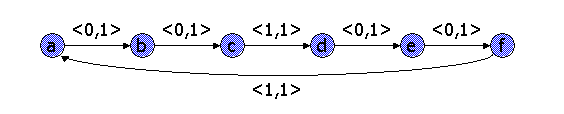
\includegraphics[width=0.5\textwidth]{p243.png}
         \caption{}
         \label{fig:p243}
\end{figure}

Construct the table of longest simple paths between each pair of nodes, in terms of T, the initiation interval. Then, for T = 4, give the constraints on (the schedule of) each pair of nodes. For any node x, let S(x) be the clock, relative to the beginning of the iteration, at which the instruction represented by node x is executed. Identify below the constraints on S(a) in terms of S(b).

 
 	\item a) 	S(b) - 3 $\leq$ S(a) $\leq$ S(b) - 1
 	\item b) 	S(b) - 1 $\leq$ S(a) $\leq$ S(b) + 3
 	\item c) 	S(b) + 1 $\leq$ S(a) $\leq$ S(b) - 3
 	\item d) 	S(b) - 3 $\leq$ S(a) $\leq$ S(b) + 1


{\color{red}Notice that there is only one simple path from any node to any other. Thus, we can compute the lengths of the longest simple paths by adding the second components of the lables, and subtracting T times the sum of the first components. Here is the table:}

$$
\begin{array}{|l|l||c||c|c|c|c|}
\hline & \mathbf{a} & \mathbf{b} & \mathbf{c} & \mathbf{d} & \mathbf{e} & \mathbf{f} \\
\hline \hline \mathbf{a} & - & 1 & 2 & 3-T & 4-T & 5-T \\
\hline \mathbf{b} & 5-2 T & - & 1 & 2-T & 3-T & 4-T \\
\hline \mathbf{c} & 4-2 T & 5-2 T & - & 1-T & 2-T & 3-T \\
\hline \mathbf{d} & 3-T & 4-T & 5-T & - & 1 & 2 \\
\hline \mathbf{e} & 2-T & 3-T & 4-T & 5-2 T & - & 1 \\
\hline \mathbf{f} & 1-T & 2-T & 3-T & 4-2 T & 5-2 T & - \\
\hline
\end{array}
$$

{\color{red}If T = 4, the values of these expressions are:

To read the constraints off of this table, suppose that the entry in the row for x and column for y is v. Also, suppose that the entry in the row for y and the column for x is u. Then the constraint on S(x) is:
S(y) + u $\leq$ S(x) $\leq$ S(y) - v

For example, S(b) - 3 $\leq$ S(a) $\leq$ S(b) - 1.


Solution : a
}



\end{problem}



\begin{problem}
Here is the sequence of instructions constituting the body of a loop that we wish to software-pipeline:

\item LD
\item ST
\item LD
\item ADD
\item ST
\item ADD
\item ST

The machine model allows each instruction to be performed in one clock tick. It also allows, in one clock tick, for the initiation of one load (LD), one store (ST), and one addition (ADD).

To form an optimal pipeline, we need to pick the shortest possible period --- the interval between initiations of successive iterations of the loop. Then, in order to make the pipeline meet the constraints of the machine, we may need to introduce delay (nop instructions) into the sequence of instructions executed by each iteration. Especially, we must avoid having the machine try to execute two or more of the same type of instruction (load, store, or add) at the same clock tick.

Your job is to find the shortest possible period, and for that period, to find the smallest number of nop's that need to be inserted. Find, in the list below, the one choice that has both the shortest possible period and the fewest nop's.

 
\item   a) 	Period = 4 with 1 delay: LD, nop, ST, LD, ADD, ST, ADD, ST
\item  	b) 	Period = 2 with 1 delay: LD, ST, nop, LD, ADD, ST, ADD, ST
\item  	c) 	Period = 3 with 2 delays: LD, ST, nop, nop, LD, ADD, ST, ADD, ST
\item  	d) 	Period = 4 with no delays: LD, ST, LD, ADD, ST, ADD, ST


{\color{red}

There are 3 store's so the period has to be at least 3. In proof: if the period is 1, then stores from three different iterations will be executed at each clock. If the period is 2, then either the odd clock ticks or the even clock ticks must have stores from two different iterations.
Now, let us see if we can find a schedule with period 3. Introducing no delay won't work. The ST in instruction 5 for iteration i will be executed in the same clock as the ST in instruction 2 for iteration i+1. Introducing only one delay won't work either. If the nop is before the first ST or after the second ST, then there is a conflict between the first two stores, of the same type as if there were no delays introduced. But if the nop is between the first and second ST's, then there is a conflict between the first and third ST's: instruction 7 from iteration i is executed at the same clock as instruction 2 from iteration i+2.

However, there are several ways to introduce two nop's so that no two instructions of the same type from the same iteration are executed on clock ticks whose numbers differ by a multiple of the period --- 3. For example, we can add two nop's between instructions 3 and 4, to get the sequence:

LD, ST, LD, nop, nop, ADD, ST, ADD, ST.

The loads occur at clocks 1 and 3 --- a difference of 2, which is not divisible by 3. The ADD's occur at clocks 6 and 8, again a difference not divisible by 3. The stores occur at clocks 2, 7, and 9, and none of the differences 9-2, 9-7, or 7-2 are divisible by 3.

Solution:c
}
\end{problem}


